\documentclass[12pt,a4paper,oneside]{book} 
\usepackage[utf8]{inputenc}
\usepackage[spanish]{babel}
\usepackage{amsmath}
\usepackage{amsfonts}
\usepackage{amssymb}
\usepackage{graphicx}
\usepackage[left=2.54cm,right=2.54cm,top=2.54cm,bottom=2.54cm]{geometry}

\begin{document}
	
	\thispagestyle{empty} 
	
	\begin{center} 
		\LARGE{UNIVERSIDAD PRIVADA DE TACNA} \\[0.5cm] \Large{FACULTAD DE INGENIERÍA DE SISTEMAS}\\[0.5cm] \large{ ESCUELA PROFESIONAL DE INGENIERÍA SISTEMAS} 
	\end{center}
	
	\begin{figure}[htb]
		\centering 
\includegraphics[width=5cm, height=7cm]{img/uptlogo.png}
	\end{figure}
	
	\begin{center} \LARGE{\bf Informe N 01:}\\ \vspace{.25cm} { 
			\Large \bfseries {CREANDO UNA BASE DE DATOS DOCUMENTAL}}\\ 
		
	\end{center}
	
	\large{\bf Curso: } Base de Datos II
	\textbf{(SI-775)}\\
	\large{\bf Docente: } Ing. Patrick Cuadros Quiroga\\
	\large{\bf Alumno: } Liendo Velásquez , Joaquin\\
	\large{\bf Codigo: } 2016054463\\
	
	
	
	\begin{center} 
		\Large \textsc{Tacna - Perú} \\
		\Large \textsc{2020 } 
	\end{center}

\newpage
\begin{itemize}
	\item {Iniciamos sesión en AWS Educate y vamos a MyClassrooms, nos saldrán las clases en las que estamos, en este caso elegiremos BD II}\\
	
	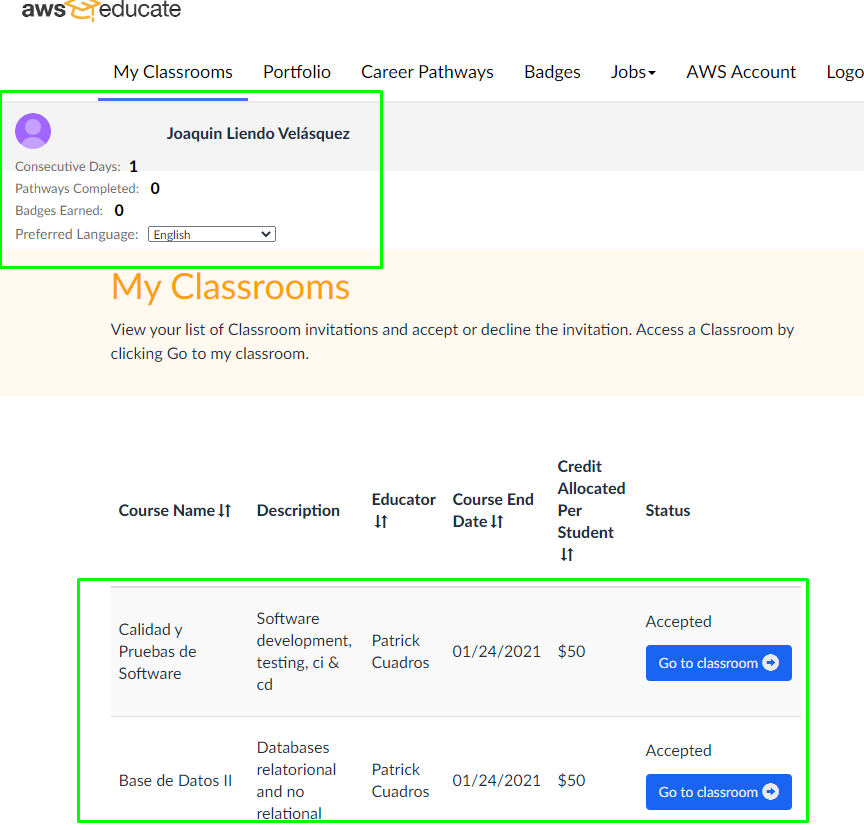
\includegraphics[width=16cm, height=10cm]{img/1.png}\\
	
	\item {Luego nos aparecerá el estado de la clase, para hacer el laboratorio elegimos AWS Console.}\\
	
	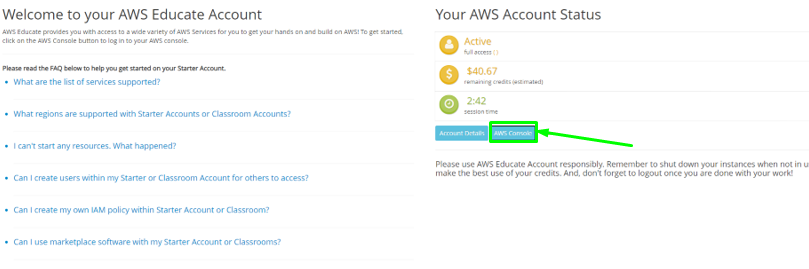
\includegraphics[width=16cm, height=6cm]{img/2.png}\\
	
\end{itemize}


\newpage
\begin{itemize}
	\item {Primero vamos a la consola.}\\
	
	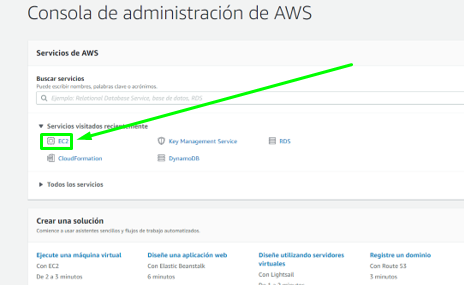
\includegraphics[width=16cm, height=10cm]{img/3.png}\\
	
	\item {Ya aquí nos vamos a Pares de claves.}\\
	
	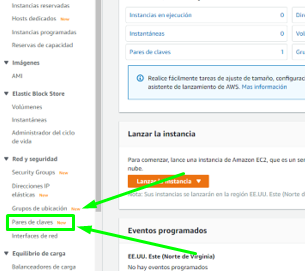
\includegraphics[width=16cm, height=10cm]{img/4.png}\\
	
\end{itemize}


\newpage
\begin{itemize}
	\item {Le damos nombre y en crear par de claves.}\\
	
	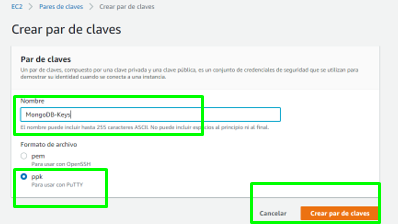
\includegraphics[width=16cm, height=10cm]{img/5.png}\\
	
	\item {Una vez creado nos descargara un archivo.}\\
	
	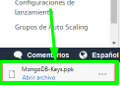
\includegraphics[width=10cm, height=5cm]{img/6.png}\\
	
\end{itemize}


\newpage
\begin{itemize}
	\item {Vamos a crear una nueva plantilla AWS, elegimos una nueva y nos redirigirá a una página para crearla.}\\
	
	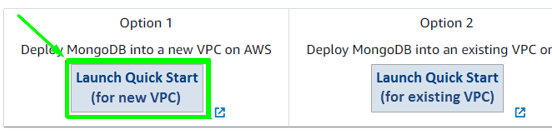
\includegraphics[width=16cm, height=7cm]{img/7.png}\\
	
	\item {En la página dejamos la parte de plantilla en como esta predeterminado. Y apretamos siguiente.}\\
	
	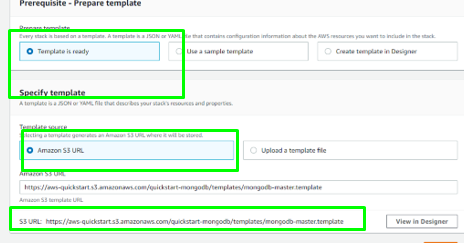
\includegraphics[width=10cm, height=12cm]{img/8.png}\\
	
\end{itemize}


\newpage
\begin{itemize}
	\item {Vamos a configurar los detalles. Primero las zonas disponibles, en este caos elegiremos las 2 primeras y en el número de zonas 2.}\\
	
	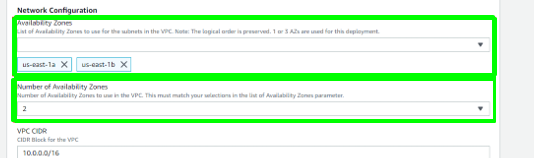
\includegraphics[width=16cm, height=7cm]{img/9.png}\\
	
	\item {Lo que viene lo dejamos por defecto.}\\
	
	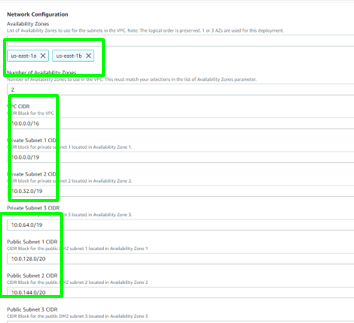
\includegraphics[width=16cm, height=12cm]{img/10.png}\\
	
\end{itemize}


\newpage
\begin{itemize}
	\item {En Allowed Bastion External Access CIDR, le ponemos una por defecto de aws vpc que seria 172.31.0.0/16}\\
	
	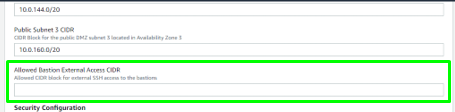
\includegraphics[width=16cm, height=5cm]{img/11.png}\\
	
	\item {Ahora configuraremos la seguridad, en Keir Pair name seleccionamos la que hemos creado con anterioridad}\\
	
	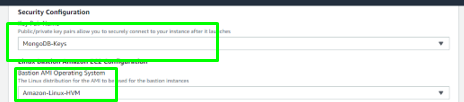
\includegraphics[width=16cm, height=3cm]{img/12.png}\\
	
	\item {Otra cosa que pasaremos a configurar será el admin username que por defecto será admin, y la contraseña, en mi caso será basededatos123}\\
	
	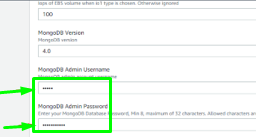
\includegraphics[width=16cm, height=4cm]{img/13.png}\\
	
\end{itemize}


\newpage
\begin{itemize}
	\item {Lo demás lo dejaríamos por defecto ya que en la mayoría de casos se ajustan a una configuración recomendada.}\\
	
	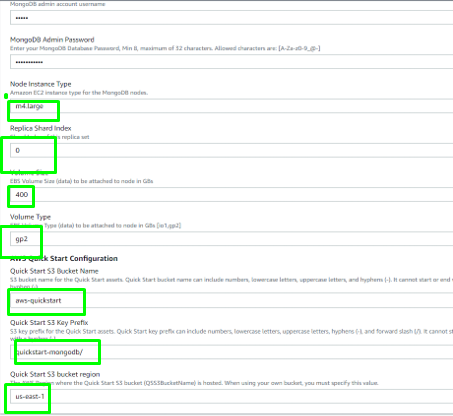
\includegraphics[width=16cm, height=10cm]{img/14.png}\\
	
	\item {Aquí puede especificar etiquetas (pares clave-valor) para los recursos en su pila y establecer opciones avanzadas. Pero no lo tocaremos por ahora así que bajamos y siguiente}\\
	
	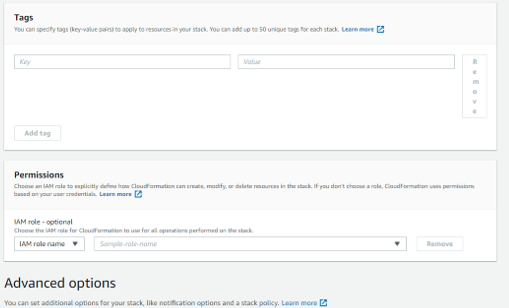
\includegraphics[width=16cm, height=8cm]{img/15.png}\\
	
	
	
\end{itemize}


\newpage
\begin{itemize}
	\item {Aquí podremos visualizar la configuración de la plantilla}\\
	
	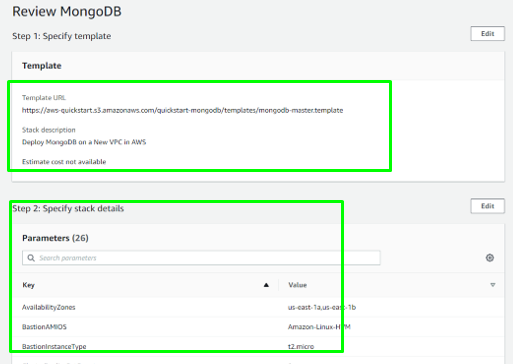
\includegraphics[width=16cm, height=10cm]{img/16.png}\\
	
	\item {Como ya terminamos le damos click en crear}\\
	
	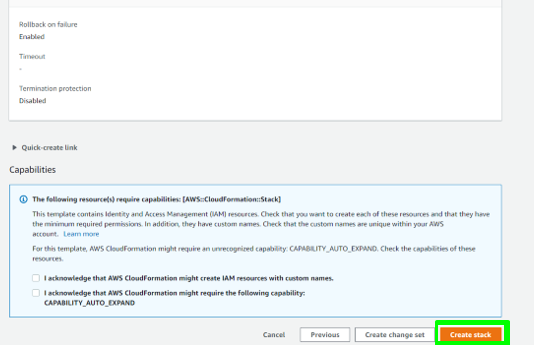
\includegraphics[width=16cm, height=8cm]{img/17.png}\\
	
	
	
\end{itemize}


\newpage
\begin{itemize}
	\item {Como vemos la creación esta en progreso}\\
	
	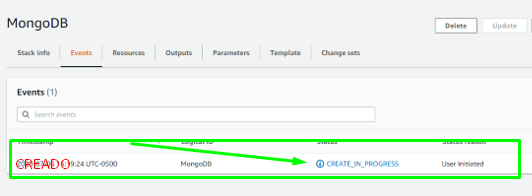
\includegraphics[width=16cm, height=10cm]{img/18.png}\\
	
	\item {Apenas esté terminada saldrá el status en CREATE\_COMPLETE}\\
	
	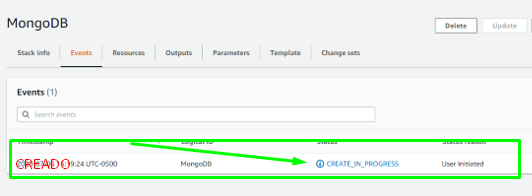
\includegraphics[width=16cm, height=8cm]{img/18.png}\\
	
	
	
\end{itemize}





	
\end{document}